\documentclass[UTF8,10pt,a4paper]{ctexart}
\usepackage[a4paper,margin=14mm,top=16mm,bottom=15mm]{geometry}
\usepackage{amsmath,amssymb}
\usepackage[version=4]{mhchem}
\usepackage{chemfig}
\usepackage{tikz}
\usetikzlibrary{calc,arrows.meta,positioning}
\usepackage{booktabs,tabularx,array,longtable,multirow}
\usepackage{enumitem}
\usepackage{graphicx}
\usepackage{fancyhdr}
\usepackage{titlesec}
\usepackage{xcolor}
\usepackage{siunitx}
\usepackage{hyperref}
\usepackage{float}
\usepackage{multicol}
\usepackage{xparse}

\definecolor{bluehead}{HTML}{174A7E}
\definecolor{ans}{HTML}{117A70}
\definecolor{orange}{HTML}{B65F12}
\definecolor{lightorange}{HTML}{FFF7EE}
\definecolor{linegray}{HTML}{C7CDD1}
\definecolor{graytext}{HTML}{5B6268}

\setlength{\parindent}{0pt}
\setlength{\parskip}{2pt}
\renewcommand{\arraystretch}{1.18}
\setlist[itemize]{leftmargin=1.45em,itemsep=1pt,topsep=1pt}
\hypersetup{colorlinks=true,linkcolor=bluehead,urlcolor=bluehead}

\newif\ifanswers
\ifdefined\ANSWERS\answerstrue\else\answersfalse\fi
\newcommand{\Edition}{\ifanswers 答案版\else 练习版\fi}
\newcommand{\A}[2][2.3cm]{\ifanswers{\color{ans}#2}\else\rule{#1}{0.4pt}\fi}
\newcommand{\AL}[2][4.0cm]{\ifanswers{\color{ans}#2}\else\rule{#1}{0.4pt}\fi}
\newcommand{\AB}[2][5.8cm]{\ifanswers{\color{ans}#2}\else\parbox[c][1.0cm][c]{#1}{\centering\rule{.88\linewidth}{0.4pt}}\fi}
\newcommand{\BlankCell}[1][1.0cm]{\ifanswers\else\rule{#1}{0.4pt}\fi}
\newcommand{\smallrule}[1]{\textcolor{graytext}{\small #1}}

\titleformat{\section}{\Large\bfseries\color{bluehead}}{\thesection}{0.55em}{}
\titleformat{\subsection}{\large\bfseries\color{bluehead}}{\thesubsection}{0.5em}{}
\titlespacing*{\section}{0pt}{8pt}{5pt}
\titlespacing*{\subsection}{0pt}{6pt}{3pt}

\pagestyle{fancy}
\fancyhf{}
\fancyhead[L]{\small 记忆默写复习回顾 06 · 立体化学}
\fancyhead[R]{\small \Edition · v5.2}
\fancyfoot[C]{\thepage}
\renewcommand{\headrulewidth}{0.35pt}

% ---------- common drawings ----------
\newcommand{\Fischer}[4]{%
\begin{tikzpicture}[baseline=-0.55ex,scale=.58]
  \draw[line width=.72pt] (0,-1.15)--(0,1.15);
  \draw[line width=.72pt] (-1.15,0)--(1.15,0);
  \node[above] at (0,1.15) {#1};
  \node[below] at (0,-1.15) {#2};
  \node[left] at (-1.15,0) {#3};
  \node[right] at (1.15,0) {#4};
\end{tikzpicture}}

\newcommand{\FischerTwo}[6]{%
\begin{tikzpicture}[baseline=-0.5ex,scale=.54]
  \draw[line width=.72pt] (0,-1.85)--(0,1.85);
  \draw[line width=.72pt] (-1.0,.62)--(1.0,.62);
  \draw[line width=.72pt] (-1.0,-.62)--(1.0,-.62);
  \node[above] at (0,1.85) {#1};
  \node[left] at (-1.0,.62) {#2}; \node[right] at (1.0,.62) {#3};
  \node[left] at (-1.0,-.62) {#4}; \node[right] at (1.0,-.62) {#5};
  \node[below] at (0,-1.85) {#6};
\end{tikzpicture}}

\newcommand{\Newman}[6]{%
\begin{tikzpicture}[baseline=-0.55ex,scale=.62]
  \draw[line width=.8pt] (0,0) circle (.47);
  \fill (0,0) circle (1.3pt);
  \foreach \ang/\lab in {90/#1,210/#2,330/#3}{\draw[line width=.72pt] (0,0)--(\ang:.94);\node at (\ang:1.20){\lab};}
  \foreach \ang/\lab in {30/#4,150/#5,270/#6}{\draw[line width=.72pt] (\ang:.47)--(\ang:.99);\node at (\ang:1.22){\lab};}
\end{tikzpicture}}

\newcommand{\TetraR}{%
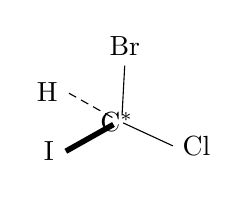
\begin{tikzpicture}[baseline=-0.55ex,scale=.68]
\node at (0,0){C$^*$};
\draw (0.1,.12)--(.15,1.05) node[above]{Br};
\draw (0.12,-.02)--(1.05,-.45) node[right]{Cl};
\draw[line width=2.0pt] (-.06,-.05)--(-.95,-.55) node[left]{I};
\draw[densely dashed] (-.08,.08)--(-.92,.55) node[left]{H};
\end{tikzpicture}}

\newcommand{\Allene}[4]{%
\begin{tikzpicture}[baseline=-0.45ex,scale=.57]
 \node at (-1.35,0){C};\node at (0,0){C};\node at (1.35,0){C};
 \draw[double distance=1.6pt] (-1.1,0)--(-.24,0);\draw[double distance=1.6pt] (.24,0)--(1.1,0);
 \draw (-1.58,.10)--(-2.18,.72) node[left]{#1}; \draw (-1.58,-.10)--(-2.18,-.72) node[left]{#2};
 \draw[densely dashed] (1.58,.05)--(2.18,.68) node[right]{#3}; \draw[line width=1.8pt] (1.58,-.05)--(2.18,-.68) node[right]{#4};
\end{tikzpicture}}

\newcommand{\SpiroSketch}{%
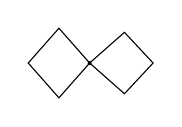
\begin{tikzpicture}[baseline=-0.4ex,scale=.52]
  \draw (-1.5,0)--(-.75,.85)--(0,0)--(-.75,-.85)--cycle;
  \draw (0,0)--(.85,.75)--(1.55,0)--(.85,-.75)--cycle;
  \fill (0,0) circle (1.4pt);
\end{tikzpicture}}

\newcommand{\BiphenylSketch}{%
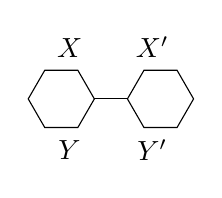
\begin{tikzpicture}[baseline=-0.4ex,scale=.42]
  \draw (0:1)--(60:1)--(120:1)--(180:1)--(240:1)--(300:1)--cycle;
  \begin{scope}[xshift=3.0cm]
    \draw (0:1)--(60:1)--(120:1)--(180:1)--(240:1)--(300:1)--cycle;
  \end{scope}
  \draw (1,0)--(2,0);
  \node[above] at (.25,.95){$X$};\node[below] at (.25,-.95){$Y$};
  \node[above] at (2.75,.95){$X'$};\node[below] at (2.75,-.95){$Y'$};
\end{tikzpicture}}

\newcommand{\CyclopropaneTwo}[2]{%
\begin{tikzpicture}[baseline=-0.45ex,scale=.62]
  \coordinate (A) at (0,1); \coordinate (B) at (-.9,-.55); \coordinate (C) at (.9,-.55);
  \draw[line width=.8pt] (A)--(B)--(C)--cycle;
  \draw[line width=1.8pt] (B)--(-1.35,-.95) node[left]{#1};
  \draw[densely dashed] (C)--(1.35,-.95) node[right]{#2};
\end{tikzpicture}}


\newcommand{\GlucoseFischer}{%
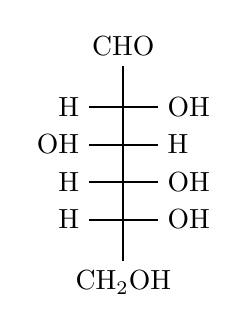
\begin{tikzpicture}[baseline=-0.5ex,scale=.46]
  \draw[line width=.72pt] (0,-2.7)--(0,2.7);
  \draw[line width=.72pt] (-.95,1.55)--(.95,1.55); \node[left] at (-.95,1.55){H}; \node[right] at (.95,1.55){OH};
  \draw[line width=.72pt] (-.95,.52)--(.95,.52); \node[left] at (-.95,.52){OH}; \node[right] at (.95,.52){H};
  \draw[line width=.72pt] (-.95,-.52)--(.95,-.52); \node[left] at (-.95,-.52){H}; \node[right] at (.95,-.52){OH};
  \draw[line width=.72pt] (-.95,-1.55)--(.95,-1.55); \node[left] at (-.95,-1.55){H}; \node[right] at (.95,-1.55){OH};
  \node[above] at (0,2.7){CHO};\node[below] at (0,-2.7){\ce{CH2OH}};
\end{tikzpicture}}

\newcommand{\DichloroTrans}{%
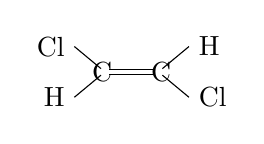
\begin{tikzpicture}[baseline=-0.45ex,scale=.52]
 \draw[double distance=1.5pt] (-.55,0)--(.55,0); \node at (-.72,0){C};\node at (.72,0){C};
 \draw (-.75,.08)--(-1.4,.62) node[left]{Cl};\draw (-.75,-.08)--(-1.4,-.62) node[left]{H};
 \draw (.75,.08)--(1.4,.62) node[right]{H};\draw (.75,-.08)--(1.4,-.62) node[right]{Cl};
\end{tikzpicture}}
\newcommand{\DichloroCis}{%
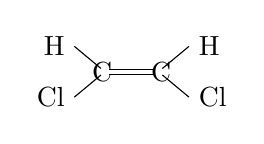
\begin{tikzpicture}[baseline=-0.45ex,scale=.52]
 \draw[double distance=1.5pt] (-.55,0)--(.55,0); \node at (-.72,0){C};\node at (.72,0){C};
 \draw (-.75,.08)--(-1.4,.62) node[left]{H};\draw (-.75,-.08)--(-1.4,-.62) node[left]{Cl};
 \draw (.75,.08)--(1.4,.62) node[right]{H};\draw (.75,-.08)--(1.4,-.62) node[right]{Cl};
\end{tikzpicture}}
\newcommand{\CyclobutaneCisThirteen}{%
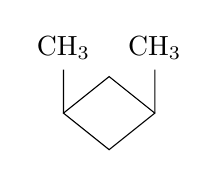
\begin{tikzpicture}[baseline=-0.45ex,scale=.58]
 \coordinate (L) at (-1,0);\coordinate (T) at (0,.8);\coordinate (R) at (1,0);\coordinate (B) at (0,-.8);
 \draw (L)--(T)--(R)--(B)--cycle;
 \draw (L)--(-1,.95) node[above]{\ce{CH3}};\draw (R)--(1,.95) node[above]{\ce{CH3}};
\end{tikzpicture}}

\newcommand{\CyclobutaneTransThirteen}{%
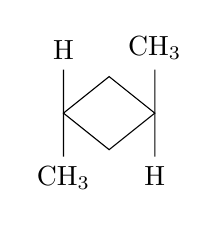
\begin{tikzpicture}[baseline=-0.45ex,scale=.58]
 \coordinate (L) at (-1,0);\coordinate (T) at (0,.8);\coordinate (R) at (1,0);\coordinate (B) at (0,-.8);
 \draw (L)--(T)--(R)--(B)--cycle;
 \draw (L)--(-1,.95) node[above]{H};\draw (L)--(-1,-.95) node[below]{\ce{CH3}};
 \draw (R)--(1,.95) node[above]{\ce{CH3}};\draw (R)--(1,-.95) node[below]{H};
\end{tikzpicture}}

\newcommand{\CyclopropaneTransRR}{%
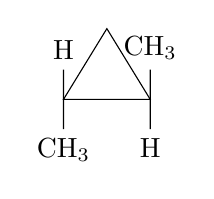
\begin{tikzpicture}[baseline=-0.45ex,scale=.58]
 \coordinate (A) at (0,1);\coordinate (L) at (-.95,-.55);\coordinate (R) at (.95,-.55);\draw (A)--(L)--(R)--cycle;
 \draw (L)--(-.95,.1) node[above]{H};\draw (L)--(-.95,-1.2) node[below]{\ce{CH3}};
 \draw (R)--(.95,.1) node[above]{\ce{CH3}};\draw (R)--(.95,-1.2) node[below]{H};
\end{tikzpicture}}
\newcommand{\CyclopropaneTransSS}{%
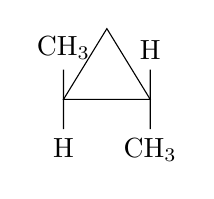
\begin{tikzpicture}[baseline=-0.45ex,scale=.58]
 \coordinate (A) at (0,1);\coordinate (L) at (-.95,-.55);\coordinate (R) at (.95,-.55);\draw (A)--(L)--(R)--cycle;
 \draw (L)--(-.95,.1) node[above]{\ce{CH3}};\draw (L)--(-.95,-1.2) node[below]{H};
 \draw (R)--(.95,.1) node[above]{H};\draw (R)--(.95,-1.2) node[below]{\ce{CH3}};
\end{tikzpicture}}
\newcommand{\CyclopropaneCisMethyl}{%
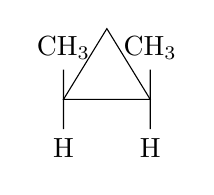
\begin{tikzpicture}[baseline=-0.45ex,scale=.58]
 \coordinate (A) at (0,1);\coordinate (L) at (-.95,-.55);\coordinate (R) at (.95,-.55);\draw (A)--(L)--(R)--cycle;
 \draw (L)--(-.95,.1) node[above]{\ce{CH3}};\draw (L)--(-.95,-1.2) node[below]{H};
 \draw (R)--(.95,.1) node[above]{\ce{CH3}};\draw (R)--(.95,-1.2) node[below]{H};
\end{tikzpicture}}
\newcommand{\ChairBase}{%
\draw[line width=.85pt] (0,0)--(1.1,-.32)--(2.15,.05)--(3.25,-.32)--(2.15,1.0)--(1.1,.58)--cycle;
\draw[line width=.85pt] (2.15,.05)--(2.15,1.0);}
\newcommand{\ChairAxialMe}{%
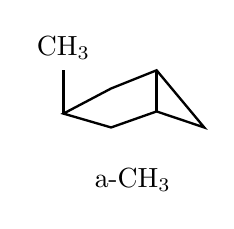
\begin{tikzpicture}[baseline=-0.45ex,scale=.55]
\ChairBase
\draw[line width=.8pt] (0,0)--(0,1.0) node[above]{\ce{CH3}};
\node[below] at (1.6,-1.05){a-\ce{CH3}};
\end{tikzpicture}}
\newcommand{\ChairEquMe}{%
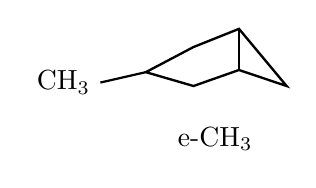
\begin{tikzpicture}[baseline=-0.45ex,scale=.55]
\ChairBase
\draw[line width=.8pt] (0,0)--(-1.05,-.24) node[left]{\ce{CH3}};
\node[below] at (1.6,-1.05){e-\ce{CH3}};
\end{tikzpicture}}
\newcommand{\ChairAxialTBu}{%
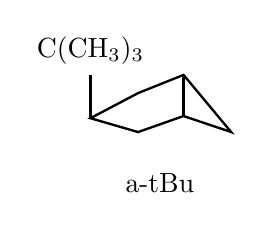
\begin{tikzpicture}[baseline=-0.45ex,scale=.55]
\ChairBase
\draw[line width=.8pt] (0,0)--(0,1.0) node[above]{\ce{C(CH3)3}};
\node[below] at (1.6,-1.05){a-tBu};
\end{tikzpicture}}
\newcommand{\ChairEquTBu}{%
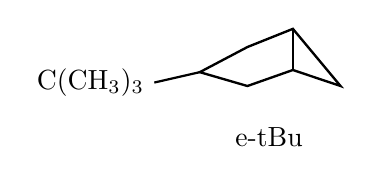
\begin{tikzpicture}[baseline=-0.45ex,scale=.55]
\ChairBase
\draw[line width=.8pt] (0,0)--(-1.05,-.24) node[left]{\ce{C(CH3)3}};
\node[below] at (1.6,-1.05){e-tBu};
\end{tikzpicture}}

\newcommand{\ChairPair}[2]{%
\begin{tikzpicture}[baseline=-0.45ex,scale=.47]
\ChairBase
\node at (-.55,.5){#1};\node at (3.65,.35){#2};
\end{tikzpicture}}

\newcommand{\Decalin}{%
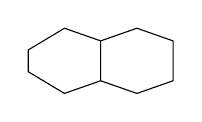
\begin{tikzpicture}[baseline=-0.5ex,scale=.46]
 \coordinate (a) at (0,0);\coordinate (b) at (1,.6);\coordinate (c) at (2,.25);\coordinate (d) at (2,-.85);\coordinate (e) at (1,-1.2);\coordinate (f) at (0,-.6);
 \coordinate (g) at (3,.6);\coordinate (h) at (4,.25);\coordinate (i) at (4,-.85);\coordinate (j) at (3,-1.2);
 \draw (a)--(b)--(c)--(d)--(e)--(f)--cycle;\draw (c)--(g)--(h)--(i)--(j)--(d);\draw (c)--(d);
\end{tikzpicture}}

\newcommand{\RuleStrip}[1]{\vspace{1mm}\noindent\colorbox{lightorange}{\parbox{\dimexpr\textwidth-2\fboxsep\relax}{\small #1}}\vspace{1mm}}


% ---------- v3 added drawings ----------
\newcommand{\CyclopropaneClMe}{%
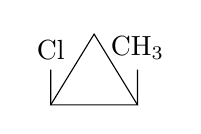
\begin{tikzpicture}[baseline=-0.45ex,scale=.58]
 \coordinate (A) at (0,1);\coordinate (L) at (-.95,-.55);\coordinate (R) at (.95,-.55);\draw (A)--(L)--(R)--cycle;
 \draw (L)--(-.95,.22) node[above]{Cl};\draw (R)--(.95,.22) node[above]{\ce{CH3}};
\end{tikzpicture}}
\newcommand{\CyclopropaneMeMeMeso}{%
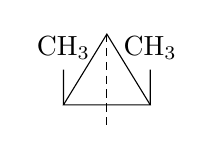
\begin{tikzpicture}[baseline=-0.45ex,scale=.58]
 \coordinate (A) at (0,1);\coordinate (L) at (-.95,-.55);\coordinate (R) at (.95,-.55);\draw (A)--(L)--(R)--cycle;
 \draw (L)--(-.95,.22) node[above]{\ce{CH3}};\draw (R)--(.95,.22) node[above]{\ce{CH3}};
 \draw[densely dashed] (A)--(0,-1.05);
\end{tikzpicture}}
\newcommand{\CycloHexDichloroRS}{%
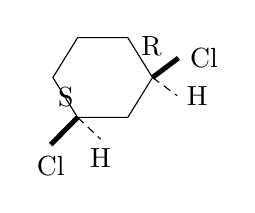
\begin{tikzpicture}[baseline=-0.45ex,scale=.55]
 \coordinate (a) at (-1.15,0);\coordinate (b) at (-.58,.92);\coordinate (c) at (.58,.92);\coordinate (d) at (1.15,0);\coordinate (e) at (.58,-.92);\coordinate (f) at (-.58,-.92);
 \draw (a)--(b)--(c)--(d)--(e)--(f)--cycle;
 \draw[line width=1.8pt] (d)--(1.75,.45) node[right]{Cl};\draw[densely dashed] (d)--(1.72,-.42) node[right]{H};
 \draw[line width=1.8pt] (f)--(-1.2,-1.55) node[below]{Cl};\draw[densely dashed] (f)--(-.05,-1.42) node[below]{H};
 \node at (1.13,.72){R};\node at (-.85,-.45){S};
\end{tikzpicture}}
\newcommand{\AlleneDichloroChiral}{\Allene{H}{Cl}{H}{Cl}}
\newcommand{\AlleneDichloroAchiral}{\Allene{H}{Cl}{H}{H}}
\newcommand{\AlkylideneCyclo}{%
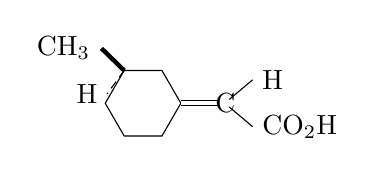
\begin{tikzpicture}[baseline=-0.45ex,scale=.48]
 \draw (0:1)--(60:1)--(120:1)--(180:1)--(240:1)--(300:1)--cycle;
 \draw[double distance=1.5pt] (1,0)--(2.0,0);\node at (2.18,0){C};
 \draw (2.28,.1)--(2.9,.62) node[right]{H};\draw (2.28,-.1)--(2.9,-.62) node[right]{\ce{CO2H}};
 \draw[line width=1.6pt] (-.5,.866)--(-1.1,1.45) node[left]{\ce{CH3}};
 \draw[densely dashed] (-.5,.866)--(-.95,.25) node[left]{H};
\end{tikzpicture}}
\newcommand{\ChairCisAE}{%
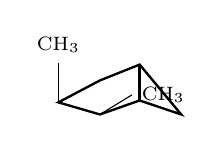
\begin{tikzpicture}[baseline=-0.45ex,scale=.48]
 \ChairBase
 \draw (0,0)--(0,1.05) node[above]{\scriptsize\ce{CH3}};
 \draw (1.1,-.32)--(1.95,.20) node[right]{\scriptsize\ce{CH3}};
\end{tikzpicture}}
\newcommand{\ChairCisEA}{%
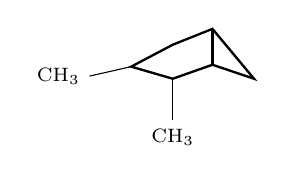
\begin{tikzpicture}[baseline=-0.45ex,scale=.48]
 \ChairBase
 \draw (0,0)--(-1.1,-.25) node[left]{\scriptsize\ce{CH3}};
 \draw (1.1,-.32)--(1.1,-1.40) node[below]{\scriptsize\ce{CH3}};
\end{tikzpicture}}
\newcommand{\ChairTransAA}{%
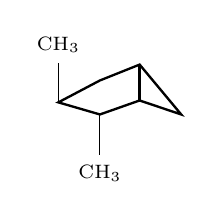
\begin{tikzpicture}[baseline=-0.45ex,scale=.48]
 \ChairBase
 \draw (0,0)--(0,1.05) node[above]{\scriptsize\ce{CH3}};
 \draw (1.1,-.32)--(1.1,-1.40) node[below]{\scriptsize\ce{CH3}};
\end{tikzpicture}}
\newcommand{\ChairTransEE}{%
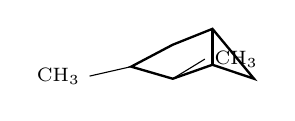
\begin{tikzpicture}[baseline=-0.45ex,scale=.48]
 \ChairBase
 \draw (0,0)--(-1.1,-.25) node[left]{\scriptsize\ce{CH3}};
 \draw (1.1,-.32)--(1.95,.20) node[right]{\scriptsize\ce{CH3}};
\end{tikzpicture}}
\newcommand{\ChairMeTBuBad}{%
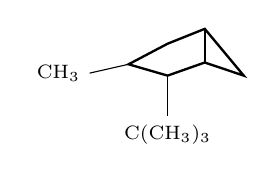
\begin{tikzpicture}[baseline=-0.45ex,scale=.45]
 \ChairBase
 \draw (0,0)--(-1.1,-.25) node[left]{\scriptsize\ce{CH3}};
 \draw (1.1,-.32)--(1.1,-1.45) node[below]{\scriptsize\ce{C(CH3)3}};
\end{tikzpicture}}
\newcommand{\ChairMeTBuFav}{%
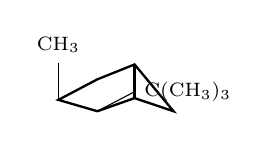
\begin{tikzpicture}[baseline=-0.45ex,scale=.45]
 \ChairBase
 \draw (0,0)--(0,1.05) node[above]{\scriptsize\ce{CH3}};
 \draw (1.1,-.32)--(2.15,.23) node[right]{\scriptsize\ce{C(CH3)3}};
\end{tikzpicture}}
\newcommand{\ChairMultiFav}{%
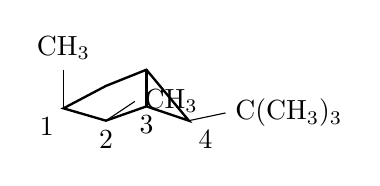
\begin{tikzpicture}[baseline=-0.45ex,scale=.49]
 \ChairBase
 % label positions roughly 1=A,2=B,3=C,4=D
 \node[below left] at (0,0){1};\node[below] at (1.1,-.32){2};\node[below] at (2.15,.05){3};\node[below right] at (3.25,-.32){4};
 \draw (0,0)--(0,1.0) node[above]{\ce{CH3}};
 \draw (1.1,-.32)--(1.85,.18) node[right]{\ce{CH3}};
 \draw (3.25,-.32)--(4.2,-.12) node[right]{\ce{C(CH3)3}};
\end{tikzpicture}}
\newcommand{\PlanarMultiCyclohexane}{%
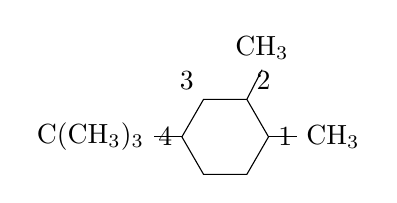
\begin{tikzpicture}[baseline=-.45ex,scale=.55]
 \foreach \a in {0,60,...,300}{\coordinate (p\a) at (\a:1);}
 \draw (p0)--(p60)--(p120)--(p180)--(p240)--(p300)--cycle;
 \node[right] at (p0){1};\node[above right] at (p60){2};\node[above left] at (p120){3};\node[left] at (p180){4};
 \draw (p0)--(1.65,0) node[right]{\ce{CH3}};
 \draw (p60)--(.85,1.55) node[above]{\ce{CH3}};
 \draw (p180)--(-1.65,0) node[left]{\ce{C(CH3)3}};
\end{tikzpicture}}
\newcommand{\ChiralCarbonGeneric}{%
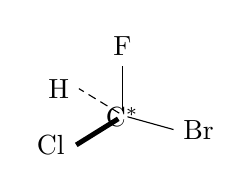
\begin{tikzpicture}[baseline=-.45ex,scale=.65]
 \node at (0,0){C$^*$};\draw (0,.12)--(0,1) node[above]{F};\draw (.1,0)--(1,-.25) node[right]{Br};\draw[line width=1.8pt] (-.08,-.04)--(-.9,-.55) node[left]{Cl};\draw[densely dashed] (-.06,.07)--(-.85,.55) node[left]{H};
\end{tikzpicture}}
\newcommand{\SawhorseDibromoA}{%
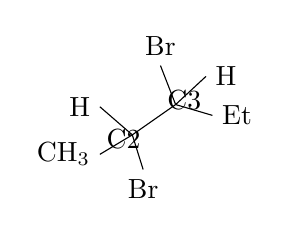
\begin{tikzpicture}[baseline=-.45ex,scale=.55]
 \draw (-.5,-.35)--(.5,.35);\node at (-.7,-.45){C2};\node at (.7,.45){C3};
 \draw (-.5,-.35)--(-1.25,.3) node[left]{H};\draw (-.5,-.35)--(-.25,-1.15) node[below]{Br};\draw (-.5,-.35)--(-1.25,-.8) node[left]{\ce{CH3}};
 \draw (.5,.35)--(1.2,1.0) node[right]{H};\draw (.5,.35)--(.15,1.25) node[above]{Br};\draw (.5,.35)--(1.35,.1) node[right]{Et};
\end{tikzpicture}}
\newcommand{\SawhorseDibromoB}{%
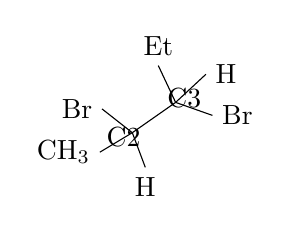
\begin{tikzpicture}[baseline=-.45ex,scale=.55]
 \draw (-.5,-.35)--(.5,.35);\node at (-.7,-.45){C2};\node at (.7,.45){C3};
 \draw (-.5,-.35)--(-1.2,.2) node[left]{Br};\draw (-.5,-.35)--(-.2,-1.15) node[below]{H};\draw (-.5,-.35)--(-1.25,-.8) node[left]{\ce{CH3}};
 \draw (.5,.35)--(1.2,1.0) node[right]{H};\draw (.5,.35)--(.1,1.2) node[above]{Et};\draw (.5,.35)--(1.35,.05) node[right]{Br};
\end{tikzpicture}}
\newcommand{\IfAns}[1]{\ifanswers #1\fi}

\setlength{\tabcolsep}{5pt}
\emergencystretch=2em
\tikzset{chemlabel/.style={fill=white,inner sep=1.1pt,outer sep=1pt}}
% v4: more spacious chair drawings; labels sit outside bonds and have white backing.
\renewcommand{\ChairCisAE}{%
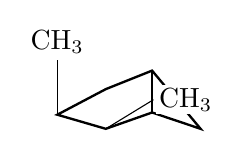
\begin{tikzpicture}[baseline=-0.45ex,scale=.56]
 \ChairBase
 \draw (0,0)--(0,1.25); \node[chemlabel,above] at (0,1.25){\ce{CH3}};
 \draw (1.1,-.32)--(2.18,.34); \node[chemlabel,right] at (2.18,.34){\ce{CH3}};
\end{tikzpicture}}
\renewcommand{\ChairCisEA}{%
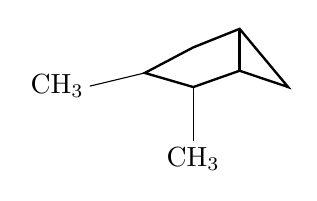
\begin{tikzpicture}[baseline=-0.45ex,scale=.56]
 \ChairBase
 \draw (0,0)--(-1.25,-.30); \node[chemlabel,left] at (-1.25,-.30){\ce{CH3}};
 \draw (1.1,-.32)--(1.1,-1.55); \node[chemlabel,below] at (1.1,-1.55){\ce{CH3}};
\end{tikzpicture}}
\renewcommand{\ChairTransAA}{%
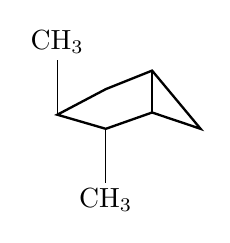
\begin{tikzpicture}[baseline=-0.45ex,scale=.56]
 \ChairBase
 \draw (0,0)--(0,1.25); \node[chemlabel,above] at (0,1.25){\ce{CH3}};
 \draw (1.1,-.32)--(1.1,-1.55); \node[chemlabel,below] at (1.1,-1.55){\ce{CH3}};
\end{tikzpicture}}
\renewcommand{\ChairTransEE}{%
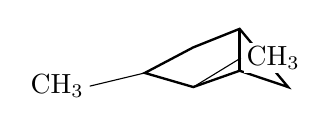
\begin{tikzpicture}[baseline=-0.45ex,scale=.56]
 \ChairBase
 \draw (0,0)--(-1.25,-.30); \node[chemlabel,left] at (-1.25,-.30){\ce{CH3}};
 \draw (1.1,-.32)--(2.18,.34); \node[chemlabel,right] at (2.18,.34){\ce{CH3}};
\end{tikzpicture}}
\renewcommand{\ChairMeTBuBad}{%
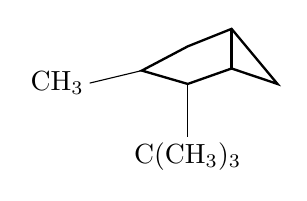
\begin{tikzpicture}[baseline=-0.45ex,scale=.53]
 \ChairBase
 \draw (0,0)--(-1.25,-.30); \node[chemlabel,left] at (-1.25,-.30){\ce{CH3}};
 \draw (1.1,-.32)--(1.1,-1.58); \node[chemlabel,below] at (1.1,-1.58){\ce{C(CH3)3}};
\end{tikzpicture}}
\renewcommand{\ChairMeTBuFav}{%
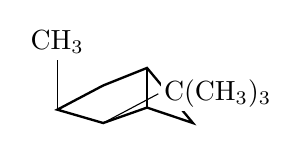
\begin{tikzpicture}[baseline=-0.45ex,scale=.53]
 \ChairBase
 \draw (0,0)--(0,1.20); \node[chemlabel,above] at (0,1.20){\ce{CH3}};
 \draw (1.1,-.32)--(2.42,.38); \node[chemlabel,right] at (2.42,.38){\ce{C(CH3)3}};
\end{tikzpicture}}
\renewcommand{\ChairMultiFav}{%
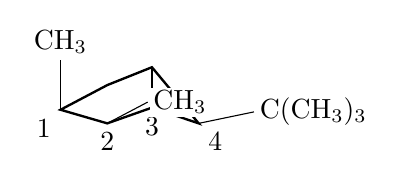
\begin{tikzpicture}[baseline=-0.45ex,scale=.54]
 \ChairBase
 \node[below left] at (0,0){1};\node[below] at (1.1,-.32){2};\node[below] at (2.15,.05){3};\node[below right] at (3.25,-.32){4};
 \draw (0,0)--(0,1.18); \node[chemlabel,above] at (0,1.18){\ce{CH3}};
 \draw (1.1,-.32)--(2.05,.18); \node[chemlabel,right] at (2.05,.18){\ce{CH3}};
 \draw (3.25,-.32)--(4.55,-.05); \node[chemlabel,right] at (4.55,-.05){\ce{C(CH3)3}};
\end{tikzpicture}}


% ---------- v5 visual refinements ----------
\tikzset{chemclear/.style={fill=white,inner sep=1.5pt,outer sep=.5pt}}

\renewcommand{\Fischer}[4]{%
\begin{tikzpicture}[baseline=-0.55ex,scale=.70]
  \draw[line width=.9pt] (0,-1.25)--(0,1.25);
  \draw[line width=.9pt] (-1.25,0)--(1.25,0);
  \node[chemclear,above] at (0,1.25) {#1};
  \node[chemclear,below] at (0,-1.25) {#2};
  \node[chemclear,left] at (-1.25,0) {#3};
  \node[chemclear,right] at (1.25,0) {#4};
\end{tikzpicture}}

\renewcommand{\FischerTwo}[6]{%
\begin{tikzpicture}[baseline=-0.55ex,scale=.62]
  \draw[line width=.9pt] (0,-2.0)--(0,2.0);
  \draw[line width=.9pt] (-1.12,.67)--(1.12,.67);
  \draw[line width=.9pt] (-1.12,-.67)--(1.12,-.67);
  \node[chemclear,above] at (0,2.0) {#1};
  \node[chemclear,left] at (-1.12,.67) {#2}; \node[chemclear,right] at (1.12,.67) {#3};
  \node[chemclear,left] at (-1.12,-.67) {#4}; \node[chemclear,right] at (1.12,-.67) {#5};
  \node[chemclear,below] at (0,-2.0) {#6};
\end{tikzpicture}}

\renewcommand{\Newman}[6]{%
\begin{tikzpicture}[baseline=-0.55ex,scale=.83]
  \draw[line width=1.0pt] (0,0) circle (.50);
  \fill (0,0) circle (1.6pt);
  \foreach \ang/\lab in {90/#1,210/#2,330/#3}{
    \draw[line width=.95pt] (0,0)--(\ang:1.02);
    \node[chemclear] at (\ang:1.36){\lab};}
  \foreach \ang/\lab in {30/#4,150/#5,270/#6}{
    \draw[line width=.95pt] (\ang:.50)--(\ang:1.08);
    \node[chemclear] at (\ang:1.39){\lab};}
\end{tikzpicture}}

\renewcommand{\TetraR}{%
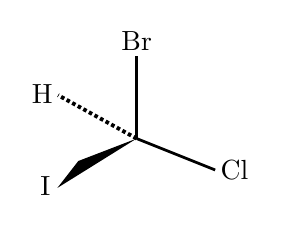
\begin{tikzpicture}[baseline=-0.55ex,scale=.95]
  \coordinate (C) at (0,0);
  \draw[line width=1.0pt] (C)--(0,1.10) node[chemclear,above]{Br};
  \draw[line width=1.0pt] (C)--(1.05,-.42) node[chemclear,right]{Cl};
  \fill (C)--(-1.06,-.66)--(-.78,-.30)--cycle;
  \node[chemclear,left] at (-1.08,-.64){I};
  \draw[line width=1.4pt,dash pattern=on 1.3pt off 1.0pt] (C)--(-1.05,.58);
  \node[chemclear,left] at (-1.05,.60){H};
\end{tikzpicture}}

\renewcommand{\ChiralCarbonGeneric}{%
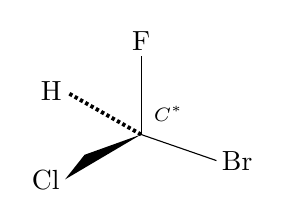
\begin{tikzpicture}[baseline=-.45ex,scale=.92]
 \coordinate (C) at (0,0);
 \draw (C)--(0,1.08) node[chemclear,above]{F};
 \draw (C)--(1.04,-.36) node[chemclear,right]{Br};
 \fill (C)--(-1.05,-.62)--(-.78,-.28)--cycle;
 \node[chemclear,left] at (-1.05,-.62){Cl};
 \draw[line width=1.4pt,dash pattern=on 1.2pt off 1pt] (C)--(-1.02,.58);
 \node[chemclear,left] at (-1.02,.60){H};
 \node[above right] at (.04,.05){\scriptsize $C^*$};
\end{tikzpicture}}

\renewcommand{\SawhorseDibromoA}{%
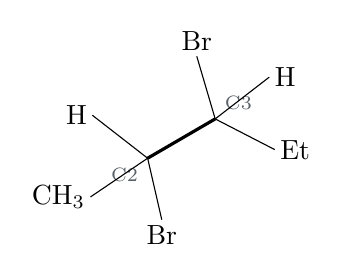
\begin{tikzpicture}[baseline=-.45ex,scale=.78]
 \coordinate (C2) at (-.55,-.32); \coordinate (C3) at (.55,.32);
 \draw[line width=1.15pt] (C2)--(C3);
 \node[graytext,below left] at (C2){\scriptsize C2}; \node[graytext,above right] at (C3){\scriptsize C3};
 \draw (C2)--(-1.45,.38) node[chemclear,left]{H};
 \draw (C2)--(-.32,-1.32) node[chemclear,below]{Br};
 \draw (C2)--(-1.48,-.95) node[chemclear,left]{\ce{CH3}};
 \draw (C3)--(.25,1.34) node[chemclear,above]{Br};
 \draw (C3)--(1.43,1.00) node[chemclear,right]{H};
 \draw (C3)--(1.52,-.18) node[chemclear,right]{Et};
\end{tikzpicture}}

\renewcommand{\SawhorseDibromoB}{%
\begin{tikzpicture}[baseline=-.45ex,scale=.78]
 \coordinate (C2) at (-.55,-.32); \coordinate (C3) at (.55,.32);
 \draw[line width=1.15pt] (C2)--(C3);
 \node[graytext,below left] at (C2){\scriptsize C2}; \node[graytext,above right] at (C3){\scriptsize C3};
 \draw (C2)--(-1.42,.30) node[chemclear,left]{Br};
 \draw (C2)--(-.30,-1.32) node[chemclear,below]{H};
 \draw (C2)--(-1.50,-.92) node[chemclear,left]{\ce{CH3}};
 \draw (C3)--(.28,1.33) node[chemclear,above]{Et};
 \draw (C3)--(1.42,.98) node[chemclear,right]{H};
 \draw (C3)--(1.52,-.18) node[chemclear,right]{Br};
\end{tikzpicture}}

\newcommand{\SawhorseDiol}{%
\begin{tikzpicture}[baseline=-.45ex,scale=.75]
 \coordinate (C2) at (.52,.58); \coordinate (C3) at (-.52,-.48);
 \draw[line width=1.15pt] (C3)--(C2);
 \node[graytext,above left] at (C2){\scriptsize C2}; \node[graytext,below right] at (C3){\scriptsize C3};
 \draw (C2)--(.12,1.62) node[chemclear,above]{H};
 \draw (C2)--(1.55,.95) node[chemclear,right]{OH};
 \draw (C2)--(1.22,-.18) node[chemclear,right]{CHO};
 \draw (C3)--(-1.50,.18) node[chemclear,left]{H};
 \draw (C3)--(.22,-.02) node[chemclear,right]{OH};
 \draw (C3)--(-.48,-1.62) node[chemclear,below]{\ce{CH2OH}};
\end{tikzpicture}}

\renewcommand{\CycloHexDichloroRS}{%
\begin{tikzpicture}[baseline=-0.45ex,scale=.72]
 \coordinate (a) at (-1.35,0);\coordinate (b) at (-.68,1.05);\coordinate (c) at (.68,1.05);
 \coordinate (d) at (1.35,0);\coordinate (e) at (.68,-1.05);\coordinate (f) at (-.68,-1.05);
 \draw[line width=1pt] (a)--(b)--(c)--(d)--(e)--(f)--cycle;
 \fill (d)--(2.02,.50)--(1.75,.18)--cycle; \node[chemclear,right] at (2.06,.50){Cl};
 \draw[line width=1.35pt,dash pattern=on 1.2pt off 1pt] (d)--(1.98,-.52); \node[chemclear,right] at (2.00,-.55){H};
 \fill (f)--(-1.32,-1.92)--(-.95,-1.54)--cycle; \node[chemclear,below left] at (-1.34,-1.92){Cl};
 \draw[line width=1.35pt,dash pattern=on 1.2pt off 1pt] (f)--(.00,-1.80); \node[chemclear,below] at (.00,-1.84){H};
 \node[font=\bfseries] at (1.25,.82){R}; \node[font=\bfseries] at (-1.04,-.58){S};
\end{tikzpicture}}

\newcommand{\ChairA}{%
 \coordinate (c1) at (1.72,-.35); \coordinate (c2) at (1.05,.72);
 \coordinate (c3) at (-.10,.35); \coordinate (c4) at (-1.18,.82);
 \coordinate (c5) at (-1.82,-.10); \coordinate (c6) at (-.66,-.58);
 \draw[line width=1.0pt] (c1)--(c2)--(c3)--(c4)--(c5)--(c6)--cycle;
 \draw[line width=2.2pt] (c5)--(c6)--(c1);}
\newcommand{\ChairB}{%
 \coordinate (c1) at (1.72,.35); \coordinate (c2) at (1.05,-.72);
 \coordinate (c3) at (-.10,-.35); \coordinate (c4) at (-1.18,-.82);
 \coordinate (c5) at (-1.82,.10); \coordinate (c6) at (-.66,.58);
 \draw[line width=1.0pt] (c1)--(c2)--(c3)--(c4)--(c5)--(c6)--cycle;
 \draw[line width=2.2pt] (c5)--(c6)--(c1);}

\renewcommand{\ChairAxialMe}{%
\begin{tikzpicture}[baseline=-.45ex,scale=.70]\ChairB
 \draw (c1)--(1.72,1.42); \node[chemclear,above] at (1.72,1.42){\ce{CH3}};
\end{tikzpicture}}
\renewcommand{\ChairEquMe}{%
\begin{tikzpicture}[baseline=-.45ex,scale=.70]\ChairA
 \draw (c1)--(2.72,.18); \node[chemclear,right] at (2.72,.18){\ce{CH3}};
\end{tikzpicture}}
\renewcommand{\ChairAxialTBu}{%
\begin{tikzpicture}[baseline=-.45ex,scale=.70]\ChairB
 \draw (c1)--(1.72,1.42); \node[chemclear,above] at (1.72,1.42){\ce{C(CH3)3}};
\end{tikzpicture}}
\renewcommand{\ChairEquTBu}{%
\begin{tikzpicture}[baseline=-.45ex,scale=.70]\ChairA
 \draw (c1)--(2.86,.18); \node[chemclear,right] at (2.86,.18){\ce{C(CH3)3}};
\end{tikzpicture}}

\renewcommand{\ChairCisAE}{%
\begin{tikzpicture}[baseline=-.45ex,scale=.72]\ChairA
 \draw (c1)--(2.67,.18); \node[chemclear,right] at (2.67,.18){\ce{CH3}};
 \draw (c2)--(1.05,1.72); \node[chemclear,above] at (1.05,1.72){\ce{CH3}};
 \node[below] at (0,-1.18){$e,a$};
\end{tikzpicture}}
\renewcommand{\ChairCisEA}{%
\begin{tikzpicture}[baseline=-.45ex,scale=.72]\ChairB
 \draw (c1)--(1.72,1.38); \node[chemclear,above] at (1.72,1.38){\ce{CH3}};
 \draw (c2)--(2.12,-.18); \node[chemclear,right] at (2.12,-.18){\ce{CH3}};
 \node[below] at (0,-1.18){$a,e$};
\end{tikzpicture}}
\renewcommand{\ChairTransAA}{%
\begin{tikzpicture}[baseline=-.45ex,scale=.72]\ChairB
 \draw (c1)--(1.72,1.38); \node[chemclear,above] at (1.72,1.38){\ce{CH3}};
 \draw (c2)--(1.05,-1.72); \node[chemclear,below] at (1.05,-1.72){\ce{CH3}};
 \node[below] at (0,-1.18){$a,a$};
\end{tikzpicture}}
\renewcommand{\ChairTransEE}{%
\begin{tikzpicture}[baseline=-.45ex,scale=.72]\ChairA
 \draw (c1)--(2.85,-.18); \node[chemclear,right] at (2.85,-.18){\ce{CH3}};
 \draw (c2)--(2.05,1.18); \node[chemclear,above right] at (2.05,1.18){\ce{CH3}};
 \node[below] at (0,-1.18){$e,e$};
\end{tikzpicture}}
\renewcommand{\ChairMeTBuBad}{%
\begin{tikzpicture}[baseline=-.45ex,scale=.67]\ChairA
 \draw (c1)--(2.67,.18); \node[chemclear,right] at (2.67,.18){\ce{CH3}};
 \draw (c2)--(1.05,1.72); \node[chemclear,above] at (1.05,1.72){\ce{C(CH3)3}};
\end{tikzpicture}}
\renewcommand{\ChairMeTBuFav}{%
\begin{tikzpicture}[baseline=-.45ex,scale=.67]\ChairB
 \draw (c1)--(1.72,1.38); \node[chemclear,above] at (1.72,1.38){\ce{CH3}};
 \draw (c2)--(2.30,-.10); \node[chemclear,right] at (2.30,-.10){\ce{C(CH3)3}};
\end{tikzpicture}}

\renewcommand{\PlanarMultiCyclohexane}{%
\begin{tikzpicture}[baseline=-.45ex,scale=.70]
 \foreach \a in {0,60,...,300}{\coordinate (p\a) at (\a:1);}
 \draw[line width=1pt] (p0)--(p60)--(p120)--(p180)--(p240)--(p300)--cycle;
 \node[right] at (p0){\scriptsize 1};\node[above right] at (p60){\scriptsize 2};
 \node[above left] at (p120){\scriptsize 3};\node[left] at (p180){\scriptsize 4};
 \draw (p0)--(1.72,0); \node[chemclear,right] at (1.72,0){\ce{CH3}};
 \draw (p60)--(.88,1.58); \node[chemclear,above] at (.88,1.58){\ce{CH3}};
 \draw (p180)--(-1.82,0); \node[chemclear,left] at (-1.82,0){\ce{C(CH3)3}};
\end{tikzpicture}}
\renewcommand{\ChairMultiFav}{%
\begin{tikzpicture}[baseline=-.45ex,scale=.72]\ChairB
 \node[below right] at (c1){\scriptsize 1};\node[below] at (c2){\scriptsize 2};
 \node[below left] at (c3){\scriptsize 3};\node[below left] at (c4){\scriptsize 4};
 \draw (c1)--(1.72,1.38); \node[chemclear,above] at (1.72,1.38){\ce{CH3}};
 \draw (c2)--(2.10,-.18); \node[chemclear,right] at (2.10,-.18){\ce{CH3}};
 \draw (c4)--(-2.25,-.48); \node[chemclear,left] at (-2.25,-.48){\ce{C(CH3)3}};
\end{tikzpicture}}

\newcommand{\DecalinBase}{%
 \coordinate (t) at (0,.55); \coordinate (b) at (0,-.55);
 \coordinate (l1) at (-.82,1.02); \coordinate (l2) at (-1.55,.55);
 \coordinate (l3) at (-1.55,-.55); \coordinate (l4) at (-.82,-1.02);
 \coordinate (r1) at (.82,1.02); \coordinate (r2) at (1.55,.55);
 \coordinate (r3) at (1.55,-.55); \coordinate (r4) at (.82,-1.02);
 \draw[line width=1pt] (t)--(l1)--(l2)--(l3)--(l4)--(b)--cycle;
 \draw[line width=1pt] (t)--(r1)--(r2)--(r3)--(r4)--(b)--cycle;
 \draw[line width=1.1pt] (t)--(b);}
\newcommand{\DecalinTrans}{%
\begin{tikzpicture}[baseline=-.45ex,scale=.78]\DecalinBase
 \fill (t)--(-.14,1.42)--(.14,1.42)--cycle; \node[chemclear,above] at (0,1.43){H};
 \draw[line width=1.4pt,dash pattern=on 1.2pt off 1pt] (b)--(0,-1.43); \node[chemclear,below] at (0,-1.43){H};
\end{tikzpicture}}
\newcommand{\DecalinCis}{%
\begin{tikzpicture}[baseline=-.45ex,scale=.78]\DecalinBase
 \fill (t)--(-.14,1.42)--(.14,1.42)--cycle; \node[chemclear,above] at (0,1.43){H};
 \fill (b)--(-.14,-1.42)--(.14,-1.42)--cycle; \node[chemclear,below] at (0,-1.43){H};
\end{tikzpicture}}

\begin{document}
\begin{center}
{\Huge\bfseries 记忆默写复习回顾 06}\\[3pt]
{\LARGE\bfseries 立体化学}\\[4pt]
{\large \Edition · v5.2 · 结构判断 + 命名 + 投影转换 + 构象 + 综合题}\\[5pt]
\rule{.88\textwidth}{.55pt}
\end{center}
\small
资料以课程 PPT 为主干，第1--8页按讨论不纳入。PPT 中出现的典型结构、命名和课堂题尽量保留；对课件没有写全、但做题必须用到的命名与判断规则作必要补充。
\normalsize

\section{手性、对称因素与光活性}

\subsection{从结构判断 $\sigma$、$i$、$C^*$、手性与光活性}
\begin{tabularx}{\textwidth}{>{\centering\arraybackslash}p{3.0cm} >{\centering\arraybackslash}p{3.1cm} *{5}{>{\centering\arraybackslash}X}}
\toprule
名称 / 结构 & 图示 & $\sigma$ & $i$ & $C^*$ & 手性 & 光活性\\\midrule
反式-1,2-二氯乙烯 & \DichloroTrans & \A[.65cm]{有} & \A[.65cm]{有} & \A[.65cm]{无} & \A[.65cm]{无} & \A[.65cm]{无}\\[1mm]
反式-1,3-二甲基环丁烷 & \CyclobutaneTransThirteen & \A[.65cm]{有} & \A[.65cm]{有} & \A[.65cm]{无} & \A[.65cm]{无} & \A[.65cm]{无}\\[1mm]
乳酸（2-羟基丙酸） & \Fischer{\ce{CO2H}}{\ce{CH3}}{H}{OH} & \A[.65cm]{无} & \A[.65cm]{无} & \A[.65cm]{1个} & \A[.65cm]{有} & \A[.65cm]{有}\\[1mm]
meso-酒石酸 & \FischerTwo{\ce{CO2H}}{H}{OH}{H}{OH}{\ce{CO2H}} & \A[.65cm]{有} & \A[.65cm]{--} & \A[.65cm]{2个} & \A[.65cm]{无} & \A[.65cm]{无}\\
\bottomrule
\end{tabularx}

\small\textbf{辨析：}手性碳 $C^*$ 是局部结构特征，分子手性是整体性质。有对称面时，镜像可与原分子重合，因此整体非手性；一个 $C^*$ 的化合物在本章范围内为手性，多个 $C^*$ 时仍要检查整个分子的对称性。\normalsize

\subsection{课堂例题}
\begin{center}
\setlength{\tabcolsep}{8mm}
\begin{tabular}{>{\centering\arraybackslash}p{6.2cm} >{\centering\arraybackslash}p{6.2cm}}
\textbf{A} & \textbf{B}\\[1mm]
\scalebox{1.15}{\DichloroTrans} & \scalebox{1.15}{\DichloroCis}\\[5mm]
\textbf{C} & \textbf{D}\\[1mm]
\scalebox{1.12}{\CyclobutaneCisThirteen} & \scalebox{1.12}{\CyclobutaneTransThirteen}
\end{tabular}
\end{center}
\begin{tabularx}{\textwidth}{c *{4}{>{\centering\arraybackslash}X}}
\toprule
 & A & B & C & D\\\midrule
$\sigma$ & \A[1cm]{有} & \A[1cm]{有} & \A[1cm]{有} & \A[1cm]{有}\\
$i$ & \A[1cm]{有} & \A[1cm]{无} & \A[1cm]{无} & \A[1cm]{有}\\
$C^*$ & \A[1cm]{无} & \A[1cm]{无} & \A[1cm]{无} & \A[1cm]{无}\\
光活性 & \A[1cm]{无} & \A[1cm]{无} & \A[1cm]{无} & \A[1cm]{无}\\
\bottomrule
\end{tabularx}

\vspace{2mm}
\textbf{课堂单选：下列化合物有手性的是}
\begin{center}
\begin{tabular}{c@{\hspace{7mm}}c@{\hspace{7mm}}c@{\hspace{7mm}}c}
\textbf{A} & \textbf{B} & \textbf{C} & \textbf{D}\\[1mm]
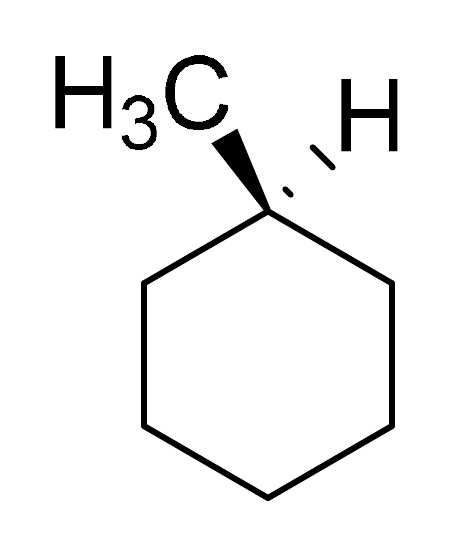
\includegraphics[width=2.9cm,height=2.65cm,keepaspectratio]{assets/p20_A.png} &
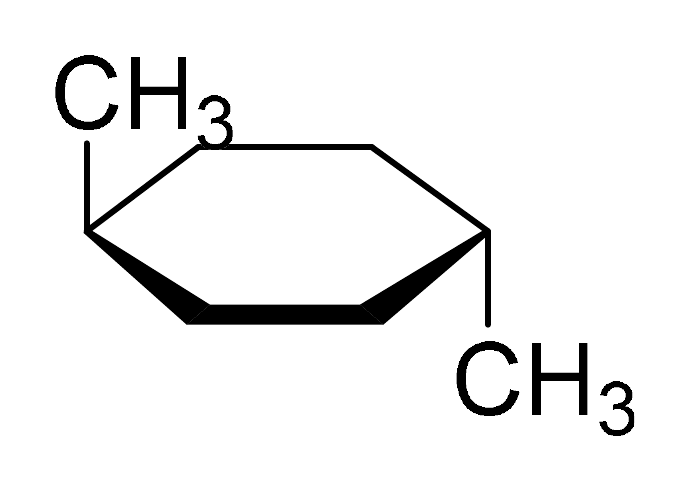
\includegraphics[width=2.9cm,height=2.65cm,keepaspectratio]{assets/p20_B.png} &
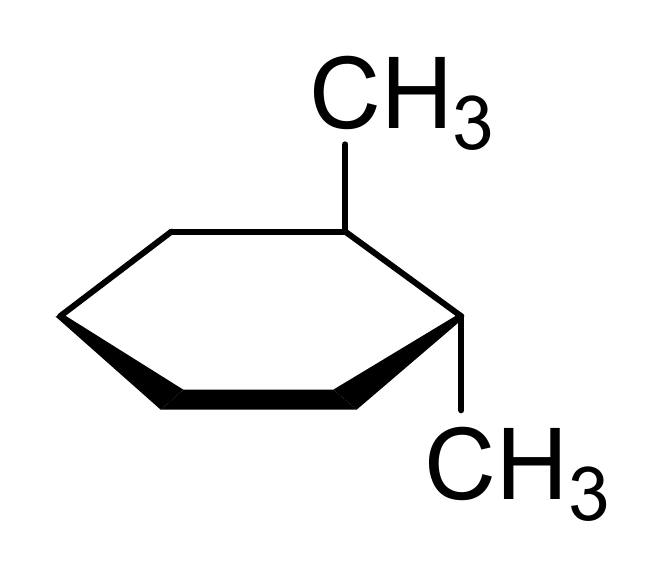
\includegraphics[width=2.9cm,height=2.65cm,keepaspectratio]{assets/p20_C.png} &
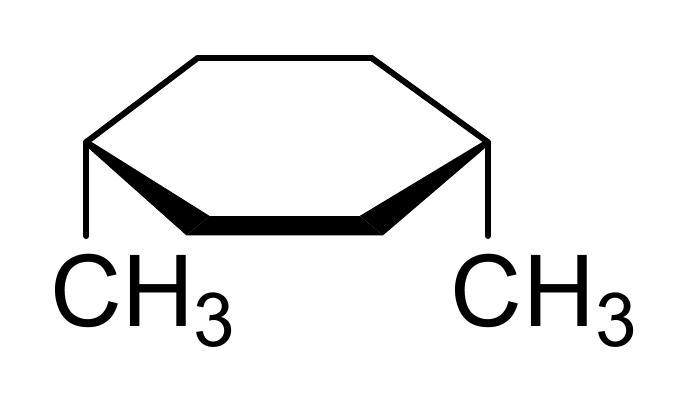
\includegraphics[width=2.9cm,height=2.65cm,keepaspectratio]{assets/p20_D.png}\\[1mm]
\multicolumn{4}{c}{答案：\A[1.5cm]{C}}
\end{tabular}
\end{center}

\subsection{乳酸与环丙烷结构}
\begin{tabularx}{\textwidth}{>{\centering\arraybackslash}p{3.1cm} >{\centering\arraybackslash}p{4.1cm} X}
\toprule
结构 & 名称 & 判断\\\midrule
\Fischer{\ce{CO2H}}{\ce{CH3}}{H}{OH} & \A[3.5cm]{乳酸（2-羟基丙酸）} & \A[6.2cm]{一个 $C^*$；手性；有一对对映体}\\[2mm]
\CyclopropaneClMe & \A[3.5cm]{1-氯-2-甲基环丙烷} & \A[6.2cm]{含手性中心；整体为手性分子}\\[2mm]
\CyclopropaneMeMeMeso & \A[3.5cm]{顺式-1,2-二甲基环丙烷} & \A[6.2cm]{有 $C^*$ 但有内部对称；非手性，meso}\\
\bottomrule
\end{tabularx}

\clearpage
\section{旋光性与构型符号}

\begin{tabularx}{\textwidth}{p{2.3cm} p{3.8cm} X p{3.2cm}}
\toprule
符号 & 表示什么 & 如何得到 & 能否只看普通结构得到\\\midrule
$R/S$ & \A[2.9cm]{绝对构型} & \A[5.0cm]{CIP 排序后按空间方向判断} & \A[2.4cm]{可以}\\
$D/L$ & \A[2.9cm]{相对构型} & \A[5.0cm]{与甘油醛参照体系比较} & \A[2.4cm]{按规则可以}\\
$+/-$（$d/l$） & \A[2.9cm]{右旋 / 左旋} & \A[5.0cm]{实验测平面偏振光的旋转方向} & \A[2.4cm]{不可以}\\
\bottomrule
\end{tabularx}

\begin{tabularx}{\textwidth}{p{3.0cm} X}
\toprule
项目 & 填写\\\midrule
右旋 & \A[10cm]{偏振平面顺时针旋转，记 $d,+$}\\
左旋 & \A[10cm]{偏振平面逆时针旋转，记 $l,-$}\\
旋光度 & \A[10cm]{实测偏转角，记 $\alpha$}\\
比旋光度 & $[\alpha]^t_D=\A[3.2cm]{\dfrac{\alpha}{lc}}$\\
$D$ 的含义 & \A[10cm]{钠光 D 线，波长 589 nm}\\
葡萄糖示例 & $[\alpha]^{20}_D=\A[2.8cm]{+52.5^\circ}$，$c=1\ \mathrm{g\,mL^{-1}}$，溶剂为 \ce{H2O}\\
\bottomrule
\end{tabularx}

\small\textbf{辨析：}同一对对映体的旋光方向相反、旋光度绝对值相同；但 $R/S$、$D/L$ 与 $+/-$ 没有固定对应关系。题目只给结构而没有实验旋光信息时，不能自行写出 $+$ 或 $-$。\normalsize

\section{楔线式与 Fischer 投影}

\subsection{书写规范}
\begin{tabularx}{\textwidth}{p{4.2cm} X}
\toprule
表示方法 & 填写\\\midrule
普通实线 & \A[8.3cm]{键在纸平面内}\\
实楔线 & \A[8.3cm]{键朝向观察者 / 纸平面前方}\\
虚楔线 & \A[8.3cm]{键远离观察者 / 纸平面后方}\\
Fischer 横线 & \A[8.3cm]{朝前}\\
Fischer 竖线 & \A[8.3cm]{朝后}\\
Fischer 交叉点 & \A[8.3cm]{代表碳原子，通常省略 C}\\
Fischer 碳链 & \A[8.3cm]{通常竖直；氧化数最高的基团放上方}\\
整体旋转 & \A[8.3cm]{$180^\circ$ 保持构型；不能把 Fischer 随意转 $90^\circ$ 后照读}\\
\bottomrule
\end{tabularx}

\small\textbf{辨析：}课件中几个“$\equiv$”表示不同画法对应同一个立体构型；要求写 Fischer 投影时应画十字并遵守“横前竖后”，不是普通平面结构式。不要为了把 H 放到竖线而任意移动或旋转基团。\normalsize

\subsection{丁-2-醇：结构、投影与完整名称}
\begin{center}
\Fischer{\ce{CH3}}{\ce{C2H5}}{H}{OH}
\qquad $\Longleftrightarrow$ \qquad
\ifanswers
\chemfig{CH_3-C(-[2]H)(-[6]C_2H_5)-OH}
\else
\fbox{\parbox[c][2.2cm][c]{5.2cm}{\centering 画对应的楔线式 / 伞形式}}
\fi
\end{center}
完整名称：\A[9cm]{丁-2-醇；判出构型后写成 $(R)$-丁-2-醇或 $(S)$-丁-2-醇。}

\clearpage
\section{CIP 次序规则与 R/S 命名}

\subsection{CIP 次序规则表}
\begin{tabularx}{\textwidth}{p{3.0cm} p{5.2cm} X}
\toprule
比较情况 & 规则 & 直接使用的例子\\\midrule
第一原子不同 & \A[4.7cm]{比较原子序数，原子序数大者优先} & $\A[5.2cm]{I>Br>Cl>F>O>N>C>D>H}$\\
同位素 & \A[4.7cm]{同位素之间比较质量数，质量数大者优先} & $\A[2.4cm]{D>H}$\\
第一原子相同 & \A[4.7cm]{比较下一层原子；把各层原子按优先级排列后逐层比较} & $\A[5.2cm]{CH_2Cl>CH_2OH;\ CO_2H>CH_3}$\\
多重键 & \A[4.7cm]{按与同一原子重复连接处理} & $\A[5.2cm]{CHO>CH_2OH;\ C{\equiv}CH>CH_3}$\\
\bottomrule
\end{tabularx}
\small\textbf{辨析：}普通元素之间比较的是\textbf{原子序数}，不是相对原子质量；只有同位素才比较质量数。\normalsize

\subsection{结构 $\rightarrow$ 排序 $\rightarrow$ R/S $\rightarrow$ 完整名称}
\begin{longtable}{>{\centering\arraybackslash}p{4.0cm} p{5.0cm} p{1.4cm} p{3.7cm}}
\toprule
结构 & 优先顺序 & 构型 & 完整名称 / 结论\\\midrule
\endfirsthead
\toprule
结构 & 优先顺序 & 构型 & 完整名称 / 结论\\\midrule
\endhead
\TetraR & \A[4.6cm]{$I>Br>Cl>H$} & \A[1cm]{R} & \A[3.7cm]{R 构型}\\[3mm]
\Fischer{\ce{CH3}}{\ce{C2H5}}{H}{OH} & \A[4.6cm]{$OH>C_2H_5>CH_3>H$} & \A[1cm]{R} & \A[3.7cm]{(R)-丁-2-醇}\\[3mm]
\Fischer{\ce{CH2Cl}}{\ce{CH2OH}}{OH}{H} & \A[4.6cm]{$OH>CH_2Cl>CH_2OH>H$} & \A[1cm]{S} & \A[3.7cm]{S 构型}\\[3mm]
\Fischer{H}{\ce{CH3}}{\ce{NH2}}{\ce{C#CH}} & \A[4.6cm]{$NH_2>C{\equiv}CH>CH_3>H$} & \A[1cm]{R} & \A[3.7cm]{R 构型}\\[3mm]
\Fischer{Ph}{$\mathrm{CH(CH_3)_2}$}{H}{\ce{CH3}} & \A[4.6cm]{$Ph>CH(CH_3)_2>CH_3>H$} & \A[1cm]{R} & \A[3.7cm]{R 构型}\\[3mm]
\bottomrule
\end{longtable}

\begin{center}
\FischerTwo{$\mathrm{CH{=}CH_2}$}{H}{\ce{NH2}}{H}{OH}{\ce{CH3}}
\end{center}
两个交叉点分别判断：上方中心 \A[1cm]{S}，下方中心 \A[1cm]{R}；完整名称：\A[7cm]{(2R,3S)-3-氨基戊-4-烯-2-醇}。

\small\textbf{Fischer 判 R/S：}最低优先级 4 在竖线上，直接按 $1\to2\to3$ 判顺逆；4 在横线上，读到的结果反转。\normalsize

\subsection{Fischer 构型专项}
\begin{center}
\begin{tabular}{>{\centering\arraybackslash}p{3.6cm} >{\centering\arraybackslash}p{3.6cm} >{\centering\arraybackslash}p{3.6cm} >{\centering\arraybackslash}p{3.6cm}}
\toprule
\Fischer{\ce{CO2H}}{H}{\ce{NH2}}{\ce{CH3}} &
\Fischer{\ce{CO2H}}{H}{\ce{CH3}}{\ce{NH2}} &
\Fischer{CHO}{\ce{CH2OH}}{H}{OH} &
\Fischer{CN}{\ce{CH3}}{OH}{H}\\
\midrule
\A[2.3cm]{R} & \A[2.3cm]{S} & \A[2.3cm]{R} & \A[2.3cm]{S}\\
\bottomrule
\end{tabular}
\end{center}

\clearpage
\section{两个手性中心：命名、对映体与 meso}

\subsection{丁-2,3-二醇}
\begin{tabularx}{\textwidth}{>{\centering\arraybackslash}p{3.2cm} >{\centering\arraybackslash}p{4.8cm} >{\centering\arraybackslash}p{3.2cm} X}
\toprule
结构 & 完整名称 & 手性 / 光活性 & 关系\\\midrule
\FischerTwo{\ce{CH3}}{OH}{H}{H}{OH}{\ce{CH3}} & \A[4.2cm]{(2R,3R)-丁-2,3-二醇} & \A[2.7cm]{手性，有光活性} & 与第二个：\A[1.7cm]{对映体}\\[3mm]
\FischerTwo{\ce{CH3}}{H}{OH}{OH}{H}{\ce{CH3}} & \A[4.2cm]{(2S,3S)-丁-2,3-二醇} & \A[2.7cm]{手性，有光活性} & 与第一个：\A[1.7cm]{对映体}\\[3mm]
\FischerTwo{\ce{CH3}}{H}{OH}{H}{OH}{\ce{CH3}} & \A[4.2cm]{meso-丁-2,3-二醇；$(2R,3S)$} & \A[2.7cm]{非手性，无光活性} & 与前两者：\A[1.7cm]{非对映体}\\
\bottomrule
\end{tabularx}

\begin{tabularx}{\textwidth}{p{5.8cm} X}
\toprule
填写 & 答案\\\midrule
$n$ 个互不等价 $C^*$ 的理论最大立体异构体数 & \A[7cm]{$2^n$}\\
丁-2,3-二醇为什么只有 3 个 & \A[7cm]{分子内部对称使 $RS$ 与 $SR$ 表示同一个 meso 化合物}\\
\bottomrule
\end{tabularx}
\small\textbf{辨析：}“手性中心相同/相似”指这些手性中心在分子中具有对称等价关系，不是在比较它们写成 R 还是 S。内部对称会使理论的 $2^n$ 数目减少。\normalsize

\subsection{赤藓糖 / 苏阿糖：四个结构}
\begin{tabularx}{\textwidth}{>{\centering\arraybackslash}X >{\centering\arraybackslash}X >{\centering\arraybackslash}X >{\centering\arraybackslash}X}
\toprule
\FischerTwo{CHO}{H}{OH}{H}{OH}{\ce{CH2OH}} &
\FischerTwo{CHO}{OH}{H}{OH}{H}{\ce{CH2OH}} &
\FischerTwo{CHO}{OH}{H}{H}{OH}{\ce{CH2OH}} &
\FischerTwo{CHO}{H}{OH}{OH}{H}{\ce{CH2OH}}\\[1mm]
\midrule
\A[3cm]{(2R,3R)，赤藓糖} & \A[3cm]{(2S,3S)，赤藓糖} & \A[3cm]{(2S,3R)，苏阿糖} & \A[3cm]{(2R,3S)，苏阿糖}\\
\bottomrule
\end{tabularx}
母体名称：\A[5cm]{2,3,4-三羟基丁醛}。

\section{Newman、锯架式与环状结构的 R/S}

\subsection{Newman：先确定 C2/C3，再判断构型}
\begin{center}
\Newman{H}{\ce{CH3}}{Cl}{\ce{CH3}}{Br}{H}
\end{center}
\begin{tabularx}{\textwidth}{p{5.2cm} X}
\toprule
问题 & 填写\\\midrule
前碳连接的基团 & \A[8cm]{H、CH$_3$、Cl；它对应主链 C3，构型 R}\\
后碳连接的基团 & \A[8cm]{H、CH$_3$、Br；它对应主链 C2，构型 S}\\
完整名称 & \A[8cm]{(2S,3R)-2-溴-3-氯丁烷}\\
\bottomrule
\end{tabularx}
\small\textbf{辨析：}Newman 的“前/后碳”只表示观察方向，不等于 C2/C3。先按系统命名确定主链编号，再把前、后两个手性中心分别对应到正确碳号。\normalsize

\subsection{锯架式：同一构型可以有不同构象}
\begin{center}
\begin{tabular}{c@{\hspace{2.0cm}}c}
\textbf{构象 A} & \textbf{构象 B}\\[1mm]
\SawhorseDibromoA & \SawhorseDibromoB
\end{tabular}
\end{center}
两个图的完整名称均为：\A[7cm]{(2R,3S)-2,3-二溴戊烷}；二者关系：\A[3cm]{构象异构体}。\\
\small\textbf{辨析：}锯架式只是换了观察与旋转方式。绕 C--C 单键转动后外观会变，但 C2、C3 的 R/S 不因此改变。\normalsize

\subsection{Fischer、锯架式、Newman 的转换}
\ifanswers
\begin{center}
\begin{tabular}{>{\centering\arraybackslash}p{4.7cm} >{\centering\arraybackslash}p{4.7cm} >{\centering\arraybackslash}p{4.7cm}}
\textbf{Fischer 投影式} & \textbf{锯架式} & \textbf{Newman 投影式}\\[1mm]
\FischerTwo{CHO}{H}{OH}{H}{OH}{\ce{CH2OH}} &
\SawhorseDiol &
\Newman{H}{OH}{CHO}{OH}{H}{\ce{CH2OH}}\\[1mm]
\multicolumn{3}{c}{\A[3cm]{同一化合物：(2R,3R)-2,3,4-三羟基丁醛}}
\end{tabular}
\end{center}
\else
\begin{center}
\FischerTwo{CHO}{H}{OH}{H}{OH}{\ce{CH2OH}}
\end{center}
\begin{tabularx}{\textwidth}{>{\centering\arraybackslash}X >{\centering\arraybackslash}X}
\toprule
改画为锯架式 & 改画为 Newman 投影式\\\midrule
\rule{0pt}{4.0cm}\rule{6.0cm}{0.4pt} & \rule{6.0cm}{0.4pt}\\
\bottomrule
\end{tabularx}
\fi
\small\textbf{检查标准：}三种画法表达的是同一个三维构型；转换以后重新检查 C2、C3 的 R/S，必须与原结构一致。\normalsize

\subsection{环状结构 R/S}
\begin{center}\resizebox{6.8cm}{!}{\CycloHexDichloroRS}\end{center}
\begin{tabularx}{\textwidth}{p{5.0cm} X}
\toprule
项目 & 填写\\\midrule
环平面处理 & \A[8cm]{可把环平面放在纸平面内，再改写成楔线式}\\
前后键 & \A[8cm]{画在环外；实楔表示一侧，虚楔表示另一侧}\\
图中构型 & \A[8cm]{一个中心 R，一个中心 S}\\
\bottomrule
\end{tabularx}
\small\textbf{辨析：}up/down、顺/反、a/e、R/S 是不同信息：up/down 表示环平面的两侧；顺/反比较两个取代基同侧还是异侧；a/e 是当前椅式中的轴向/赤道向；R/S 是绝对构型。\normalsize

\clearpage
\section{D/L 相对构型}
\begin{center}
\begin{tabular}{>{\centering\arraybackslash}p{3.1cm} >{\centering\arraybackslash}p{3.1cm} >{\centering\arraybackslash}p{3.1cm} >{\centering\arraybackslash}p{3.1cm}}
\toprule
\Fischer{CHO}{\ce{CH2OH}}{H}{OH} & \Fischer{CHO}{\ce{CH2OH}}{OH}{H} & \Fischer{\ce{CO2H}}{\ce{CH3}}{H}{OH} & \Fischer{\ce{CO2H}}{\ce{CH3}}{OH}{H}\\
\midrule
\A[2.7cm]{D-(+)-甘油醛} & \A[2.7cm]{L-(-)-甘油醛} & \A[2.7cm]{D-(-)-乳酸} & \A[2.7cm]{L-(+)-乳酸}\\
\bottomrule
\end{tabular}
\end{center}

\begin{center}
\Fischer{CHO}{\ce{CH2OH}}{H}{OH}
$\xrightarrow{[O]}$
\Fischer{\ce{CO2H}}{\ce{CH2OH}}{H}{OH}
$\xrightarrow{[H]}$
\Fischer{\ce{CO2H}}{\ce{CH3}}{H}{OH}
\end{center}
依次为：\A[10cm]{D-(+)-甘油醛、D-(-)-甘油酸、D-(-)-乳酸。}

\textbf{D-葡萄糖：}\quad \GlucoseFischer \quad 距离羰基最远的手性中心 OH 在 \A[1.4cm]{右侧}，属于 \A[1.1cm]{D} 系列。

\small\textbf{辨析：}D/L 是相对构型；$+/-$ 是实验旋光方向。D 可以是 $+$ 也可以是 $-$，L 也同样如此；不要用 D/L 推出旋光方向，也不要用 R/S 推出旋光方向。\normalsize

\textbf{单选：下列说法正确的是}\par
\begin{tabularx}{\textwidth}{c X}
A & 有手性碳的化合物一定是手性的\\
B & R 构型的化合物一定是右旋的\\
C & D/L 构型与 R/S 构型无固定对应关系\\
D & 右旋化合物的手性碳一定是 S 构型\\
\end{tabularx}
答案：\A[1.4cm]{C}。

\section{对映体、外消旋体、内消旋体、非对映体}

\subsection{酒石酸：三个结构同时判断}
\begin{tabularx}{\textwidth}{>{\centering\arraybackslash}p{3.0cm} >{\centering\arraybackslash}p{3.0cm} >{\centering\arraybackslash}p{3.0cm} X}
\toprule
I & II & III & 填写\\\midrule
\FischerTwo{\ce{CO2H}}{H}{OH}{OH}{H}{\ce{CO2H}} &
\FischerTwo{\ce{CO2H}}{OH}{H}{H}{OH}{\ce{CO2H}} &
\FischerTwo{\ce{CO2H}}{H}{OH}{H}{OH}{\ce{CO2H}} &
I：\A[3cm]{(R,R)-(+)-酒石酸}\\[2mm]
& & & II：\A[3cm]{(S,S)-(-)-酒石酸}\\
& & & III：\A[3cm]{meso-(R,S)-酒石酸}\\
& & & I / II：\A[3cm]{对映体}\\
& & & I / III：\A[3cm]{非对映体}\\
& & & II / III：\A[3cm]{非对映体}\\
\bottomrule
\end{tabularx}

\subsection{四类关系与性质}
\begin{tabularx}{\textwidth}{p{2.8cm} p{5.0cm} X}
\toprule
名称 & 结构 / 组成 & 结论\\\midrule
单一对映体 & 如 $(R)$-2-溴丁烷 & \A[5.8cm]{纯物质；手性；其 $+/-$ 由实验确定}\\
外消旋体 & \A[4.3cm]{一对对映体 1:1 混合} & \A[5.8cm]{混合物；旋光相互抵消，净旋光度 0；可拆分}\\
内消旋体 & 如 meso-酒石酸 / meso-丁-2,3-二醇 & \A[5.8cm]{单一化合物；有 $C^*$ 但整体内部对称；非手性}\\
非对映体 & 如 $(R,R)$-酒石酸与 meso-酒石酸 & \A[5.8cm]{两个非镜像立体异构体之间的关系；各自都可以是纯物质}\\
\bottomrule
\end{tabularx}

\small\textbf{辨析：}外消旋体的“无旋光”来自两种对映体等量混合后的相互抵消；内消旋体不是混合物，而是一个本身就非手性的单一化合物。非对映体不是一种混合物名称，而是两个立体异构体之间的关系。\normalsize

\subsection{对映体与非对映体的性质}
\begin{tabularx}{\textwidth}{p{3.0cm} X}
\toprule
比较 & 结论\\\midrule
一对对映体，非手性环境 & \A[10cm]{mp、bp、溶解度、普通 NMR/IR、与非手性试剂的反应速度等相同}\\
一对对映体，手性环境 / 偏振光 & \A[10cm]{可被区分；旋光方向相反且绝对值相同；与手性试剂反应速率可不同}\\
非对映体 & \A[10cm]{物理性质通常不同，反应性质也可不同，因此可利用性质差异分离}\\
\bottomrule
\end{tabularx}
\small\textbf{辨析：}“非手性环境”本身不区分一对镜像构型；加入手性试剂、手性催化剂或手性色谱环境后，二者可表现不同。\normalsize

\subsection{2-溴丁烷与乳酸}
\textbf{2-溴丁烷外消旋体：}
\begin{center}
\Fischer{\ce{CH3}}{\ce{C2H5}}{H}{Br}\quad + \quad \Fischer{\ce{CH3}}{\ce{C2H5}}{Br}{H}
\qquad \A[4.3cm]{$(\pm)$-2-溴丁烷；两种对映体各 50\%}
\end{center}

\textbf{乳酸：}
\begin{center}
\Fischer{\ce{CO2H}}{\ce{CH3}}{H}{OH}\qquad
\Fischer{\ce{CO2H}}{\ce{CH3}}{OH}{H}
\end{center}
分别为：\A[8cm]{(S)-(+)-乳酸 与 (R)-(-)-乳酸；外消旋乳酸为二者等量混合。}

\section{不含手性碳原子的对映异构}
\begin{tabularx}{\textwidth}{>{\centering\arraybackslash}p{4.2cm} p{5.0cm} X}
\toprule
结构 & 判断依据 & 结论\\\midrule
\Allene{$a$}{$b$}{$c$}{$d$} & \A[4.6cm]{$a\neq b$ 且 $c\neq d$；丙二烯两端取代基所在平面互相垂直} & \A[3.3cm]{可产生轴手性 / 对映异构}\\[3mm]
\AlleneDichloroChiral & \A[4.6cm]{1,3-二氯丙二烯；两端各有两种不同基团} & \A[3.3cm]{手性；实物与镜像不能重合}\\[3mm]
\AlleneDichloroAchiral & \A[4.6cm]{一端两个取代基相同，出现对称面} & \A[3.3cm]{非手性}\\[3mm]
\SpiroSketch & \A[4.6cm]{螺环的空间排列可使实物与镜像不能重合} & \A[3.3cm]{无普通 $C^*$ 也可手性}\\[3mm]
\BiphenylSketch & \A[4.6cm]{$2,2'$、$6,6'$ 位大基团阻碍两个苯环自由旋转} & \A[3.3cm]{可出现阻转轴手性}\\[3mm]
\AlkylideneCyclo & \A[4.6cm]{亚烷基环烷烃的空间固定可形成手性} & \A[3.3cm]{可有旋光性}\\
\bottomrule
\end{tabularx}
\small\textbf{辨析：}“有 $C^*$”不是分子手性的必要条件。丙二烯 $\mathrm{C=C=C}$ 中两个累计双键仍然是两个双键，手性来自两端取代基平面的空间关系，不能把它简化成“一根键”。\normalsize

\section{取代环烷烃：顺反、R/S 与手性}
\begin{tabularx}{\textwidth}{p{3.0cm} X}
\toprule
类型 & 判断内容\\\midrule
碳架异构 & \A[10cm]{环的大小、取代基连接位置等不同}\\
顺反异构 & \A[10cm]{取代基位于环平面的同侧 / 异侧}\\
对映异构 & \A[10cm]{同一顺反关系下仍可能出现一对镜像不重合的构型}\\
\bottomrule
\end{tabularx}

\subsection{1,2-二甲基环丙烷}
\begin{tabularx}{\textwidth}{>{\centering\arraybackslash}p{3.8cm} >{\centering\arraybackslash}p{4.4cm} >{\centering\arraybackslash}p{2.8cm} X}
\toprule
结构 & 完整名称 & 手性 & 关系\\\midrule
\CyclopropaneTransRR & \A[4.0cm]{(1R,2R)-反式-1,2-二甲基环丙烷} & \A[2.2cm]{手性} & 与下一项：\A[1.6cm]{对映体}\\[3mm]
\CyclopropaneTransSS & \A[4.0cm]{(1S,2S)-反式-1,2-二甲基环丙烷} & \A[2.2cm]{手性} & 与上一项：\A[1.6cm]{对映体}\\[3mm]
\CyclopropaneCisMethyl & \A[4.0cm]{顺式-1,2-二甲基环丙烷} & \A[2.2cm]{非手性} & \A[3.0cm]{有内部对称，meso}\\
\bottomrule
\end{tabularx}
\small\textbf{辨析：}两个反式结构都可以叫“反-1,2-二甲基环丙烷”，但这个名称不能区分它们是哪一个对映体；要唯一指出具体构型，需要再写 R/S。环状顺反用顺式/反式，不用 E/Z 代替。\normalsize

\begin{tabularx}{\textwidth}{p{5.0cm} X}
\toprule
规则 & 填写\\\midrule
判断环状分子的手性 & \A[8cm]{可把环近似看作平面，检查 $\sigma$、$i$ 以及整体镜像能否重合}\\
偶数环对位取代 & \A[8cm]{课程结论：一般无手性，只存在顺反异构}\\
相同双取代的顺式异构体 & \A[8cm]{课程结论：可为内消旋体，非手性}\\
\bottomrule
\end{tabularx}

\clearpage
\section{环己烷衍生物的构象}
\subsection{a/e、环翻转与 1,3-二轴相互作用}
\begin{tabularx}{\textwidth}{p{3.7cm} X}
\toprule
项目 & 填写\\\midrule
a 键 & \A[9cm]{axial，轴向 / 竖键；相邻碳上下交替}\\
e 键 & \A[9cm]{equatorial，赤道向；大体向环外伸展}\\
环翻转 & \A[9cm]{$a\leftrightarrow e$，但每个取代基 up/down 不变，因此顺/反关系不变}\\
1,3-二轴相互作用 & \A[9cm]{a 位取代基与同侧 C3、C5 轴向 H / 基团产生空间排斥}\\
优势构象 & \A[9cm]{能量更低、更稳定、平衡时比例更高的构象}\\
\bottomrule
\end{tabularx}
\small\textbf{辨析：}顺/反判断的是两个取代基同侧还是异侧；a/e 判断的是当前椅式中的键方向。环翻转会交换 a/e，但不会改变每个取代基的 up/down，因此也不会改变顺/反关系。\normalsize

\begin{tabularx}{\textwidth}{p{4.0cm} X}
\toprule
Newman 术语 & 与稳定性的关系\\\midrule
对位交叉（anti） & \A[8.5cm]{大基团二面角约 $180^\circ$，距离较远，较稳定}\\
邻位交叉（gauche） & \A[8.5cm]{大基团二面角约 $60^\circ$，距离较近，排斥较大}\\
\bottomrule
\end{tabularx}

\subsection{单取代环己烷}
\begin{center}
\begin{tabular}{>{\centering\arraybackslash}p{5.0cm} >{\centering\arraybackslash}p{5.0cm} >{\centering\arraybackslash}p{4.0cm}}
\toprule
a（轴向）构象 & e（赤道向）构象 & 判断\\\midrule
\ChairAxialMe & \ChairEquMe & 甲基环己烷：\A[1.2cm]{e} 构象占优势；室温约 \A[1.2cm]{95\%}\\[7mm]
\ChairAxialTBu & \ChairEquTBu & 叔丁基环己烷：\A[1.2cm]{e} 构象几乎完全占优势\\
\bottomrule
\end{tabular}
\end{center}

\subsection{二取代环己烷：顺式 / 反式与环翻转}
\textbf{顺式-1,2-二甲基环己烷（两个取代基同侧）}
\begin{center}
\ChairCisAE\qquad$\Longleftrightarrow$\qquad\ChairCisEA
\end{center}
两个构象分别为 \A[2.4cm]{$e,a$} 与 \A[2.4cm]{$a,e$}；能量关系：\A[3.0cm]{相等}。

\vspace{2mm}
\textbf{反式-1,2-二甲基环己烷（两个取代基异侧）}
\begin{center}
\ChairTransAA\qquad$\Longleftrightarrow$\qquad\ChairTransEE
\end{center}
两个构象分别为 \A[2.4cm]{$a,a$} 与 \A[2.4cm]{$e,e$}；优势构象：\A[3.0cm]{$e,e$}。

\vspace{2mm}
\textbf{顺式-1-甲基-2-叔丁基环己烷}
\begin{center}
\ChairMeTBuBad\qquad$\Longleftrightarrow$\qquad\ChairMeTBuFav
\end{center}
体积较大的叔丁基处于 \A[1.6cm]{e} 键时更稳定，因此右侧 / 对应构象为优势构象。

\subsection{多取代环己烷}
\begin{center}
\PlanarMultiCyclohexane \qquad $\Longrightarrow$ \qquad
\ifanswers \ChairMultiFav \else \fbox{\parbox[c][3.2cm][c]{7.6cm}{\centering 按原碳编号和每个取代基的 up/down 关系装入椅式；再画环翻转构象并比较稳定性}} \fi
\end{center}
判断：\A[12cm]{先比较 e 位取代基的数量；若数量相同，让体积较大的基团处于 e。}

\section{十氢萘}
系统名称：\A[8cm]{二环[4.4.0]癸烷}。

\begin{center}
\begin{tabular}{>{\centering\arraybackslash}p{6.3cm} >{\centering\arraybackslash}p{6.3cm}}
\toprule
反式十氢萘 & 顺式十氢萘\\\midrule
\DecalinTrans & \DecalinCis\\[2mm]
\A[4.8cm]{$e,e$-稠合；较稳定} & \A[4.8cm]{$e,a$-稠合；较不稳定}\\
\bottomrule
\end{tabular}
\end{center}
结论：\A[7cm]{反式十氢萘稳定性 $>$ 顺式十氢萘。}

\clearpage
\section{自由基氯代中的立体化学}
\[
\ce{CH3CH2CH2CH3 + Cl2}\xrightarrow{h\nu}\text{一氯代产物}
\]
\begin{tabularx}{\textwidth}{p{5.2cm} X}
\toprule
问题 & 填写\\\midrule
一氯代构造异构体 & \A[8.3cm]{1-氯丁烷、2-氯丁烷}\\
若把立体异构体分开计数 & \A[8.3cm]{1-氯丁烷、$(R)$-2-氯丁烷、$(S)$-2-氯丁烷，共 3 种}\\
伯氢 / 仲氢 / 叔氢相对反应活性 & \A[8.3cm]{$1:3.7:5$}\\
1-氯丁烷约占 & \A[8.3cm]{$\dfrac{6\times1}{6\times1+4\times3.7}\times100\%\approx28.8\%$}\\
2-氯丁烷约占 & \A[8.3cm]{约 $71.2\%$}\\
2-氯丁烷是否有手性 & \A[8.3cm]{有；C2 连接 Cl、H、CH$_3$、C$_2$H$_5$}\\
所得 2-氯丁烷样品是否旋光 & \A[8.3cm]{不旋光；R/S 等量生成，为外消旋体}\\
原因 & \A[8.3cm]{中间碳自由基近似平面，Cl 可从两面进攻，非手性条件下两面对等}\\
\bottomrule
\end{tabularx}
\small\textbf{辨析：}“2-氯丁烷分子有手性”和“这一瓶反应产物没有净旋光性”并不矛盾：前者说单个分子的结构，后者说样品中 R/S 两种对映体等量混合后的宏观结果。\normalsize

\section{外消旋体的拆分}
\subsection{化学拆分}
\[
(\pm)\text{酸}+(+)\text{胺}\longrightarrow
\begin{cases}
(+)\text{酸}\cdot(+)\text{胺盐}\\
(-)\text{酸}\cdot(+)\text{胺盐}
\end{cases}
\]
两种盐之间为：\A[3cm]{非对映体}；利用 \A[5cm]{溶解度、结晶等物理性质差异} 分开，再加酸释放各单一对映体。

\small\textbf{辨析：}直接分离对映体困难，是因为它们在非手性环境中的常规性质很接近；与单一手性拆分剂反应后变成非对映体，才产生可用于分离的性质差异。\normalsize

\subsection{诱导结晶}
在外消旋体过饱和溶液中加入少量纯光学异构体晶种，与晶种 \A[3.2cm]{相同构型} 的异构体优先析出。

\end{document}
